\documentclass[withindex, glossary]{cam-thesis}
\pdfminorversion=7

\usepackage[spanish]{babel}
\usepackage[utf8]{inputenc}
\usepackage[T1]{fontenc}
\usepackage[table]{xcolor}
\usepackage{multirow}
\usepackage{tabularx}
\usepackage{graphicx}
\usepackage{lmodern}
\usepackage{cleveref}

\usepackage{hyperref}
\addto\extrasspanish{%
    \def\chapterautorefname{capítulo}%
}

\usepackage{svg}
\usepackage{multicol}
\usepackage{mathtools}
\usepackage{booktabs}
\usepackage{bookmark}
\usepackage{blkarray, bigstrut}
%\usepackage{subcaption}
\usepackage{pgfgantt}
\usepackage{array}
\usepackage[capposition=top]{floatrow}

\usepackage[backend=biber, style=ieee, sorting=ynt]{biblatex}
\addbibresource{thesis.bib}

\usepackage{minted}
\usemintedstyle{manni}

\usepackage{csquotes}

\usepackage{tikz}
\usetikzlibrary{shapes.geometric, arrows.meta, fit, backgrounds, positioning, matrix, decorations.pathreplacing, calc}
\tikzstyle{startstop} = [rectangle, rounded corners, minimum width=3cm, minimum height=1cm,text centered, draw=black, fill=red!50]
\tikzstyle{io} = [trapezium, trapezium left angle=70, trapezium right angle=110, minimum width=3cm, minimum height=1cm, text centered, draw=black, fill=blue!30]
\tikzstyle{process} = [rectangle, minimum width=3cm, minimum height=1cm, text centered, draw=black, fill=orange!30]
\tikzstyle{decision} = [diamond, minimum width=3cm, minimum height=1cm, text centered, draw=black, fill=green!20]
\tikzstyle{database} = [cylinder, minimum width=3cm, minimum height=2cm, text centered, shape border rotate=90, aspect=0.25, draw=black, fill=yellow!30]
\tikzstyle{arrow} = [thick, ->, >=stealth]
\tikzstyle{line} = [-Latex]
\newcommand{\inline}[2]{%
    \begin{tikzpicture}[baseline=(word.base), txt/.style={shape=rectangle, inner sep=0pt}]
        \node[txt] (word) {\texttt{#1}};
        \node[above] at (word.north) {\footnotesize{#2}};
    \end{tikzpicture}%
}

\usepackage{pgfplots}
\pgfplotsset{compat=newest}

\setlength{\columnseprule}{0.4pt}

\title{Estudio sobre Sistemas de Antialiasing}
\author{Hugo Ferrando Seage}
\college{U-Tad}
\submissiondate{septiembre 2018\\Director: Alberto Sánchez Campos}
\date{July 2018}
\fecha{julio 2018}

% PDF meta-info
\subjectline{Máster en Computación Gráfica y Simulación}
% max 6
\keywords{opengl antialiasing temporal}

% Abstract
\espabstract{%
    Debido a la resolución limitada de las pantallas al rasterizar gráficos 3D se deforman ciertas lineas y curvas. Este fenómeno se llama aliasing. La demanda de gráficos cada vez más realistas ha propiciado la creación de diferentes técnicas y algoritmas para disimular estos defectos, sin tener que recurrir necesariemente a pantallas de mayor resolución.

    El antialiasing se ha vuelto una técnica crucial para mejorar la calidad de imagen en el software con gráficos tridimensionales. Este campo de la computación gráfica lleva años desarrollandose, con nuevas técnicas publicadas continuamente.

    Este proyecto tiene como objetivo el analisis de las distintas técnicas inventadas y la implementación de un algoritmo de temporal antialiasing, compatible con motores con deferred shading y comparable en calidad al multisampling, junto a otras propiedades.
}

\abstract{%
    When rasterizing 3D graphics using computer screens, due to their limited resolution some lines and curves will become deformed. This phenomena is called aliasing. The ever increasing demand for more realistic graphics has driven the creation of new techniques and algorithms to hide these artifacts, without necessarily using higher resolution screens.

    Antialiasing has become a crucial technique to advance image quality in graphics software. This field has been explored for years, with new approaches being developed continually.

    This projects aims to analyze different antialiasing techniques developed and the implementation of a temporal antialiasing technique, compatible with deferred shading engines and with similar quality to mutlisampling, amongst other benefits.
}

% Glossary

% Acronyms

% Contents
\begin{document}
\frontmatter{}

% Thesis body:
\chapter{Introducción}
\section{¿Qué es el aliasing?}

El antialiasing es la deformación de ciertos elementos gráficos al ser rasterizados y plasmados en una pantalla con una resolución finita. Normalmente los bordes de la geometría que tengan angulos que no se alineen perfectamente con los pixels presentaran bordes de sierra abruptos, que no es fiel a la escena como se vería de forma natural.

Este proyecto se centra en aliasing dentro del campo de la computación gráfica, pero afecta a otras disciplinas, como el procesamiento de señales (por ejemplo al digitalizar señales de audio analógicas). En general, al representar valores continuos en algún medio discreto siempre habrá algún defecto de este tipo.

Existen otros tipos de aliasing, como en el interior de texturas o al mover la camera rápidamente.

\section{¿Qué es el antialiasing?}

El antialiasing es el conjunto de técnicas cuyo objetivo es el de disimular o eliminar estas imperfecciones.

\chapter{Problemas}

\section{Aliasing en bordes de geometría}
imagen

\section{Aliasing de texturas}
Posibles soluciones: Mip Maps, LoD

\section{Specular Aliasing}
\section{Motion Aliasing}
Explicar motion blur en camaras

Accumulation motion blur (ps2+)
Per pixel motion blur (ps3+)
Per object motion blur (ps3+)

\chapter{Técnicas}

\section{Supersampling Antialiasing}

El supersampling consiste en minimizar el aliasing usando imagenes con una resolución mayor a la usada para su visualización (antialiasing espacial). Cada píxel en la pantalla será representado por más de un píxel en la imagen. Para el color final normalmente se hace la media del valor de los colores de los multiples pixels.

Estas técnicas consumen más ancho de banda y memoría, ya que los buffers tienen que guardar más información por píxel que la imagen original.

La calidad del supersampling viene dado por la cantidad de samples por pixel y la técnica para saber que pixels usar en la imagen con mayor resolución para cada pixel de la pantalla.

http://www.x86-secret.com/articles/divers/v5-6000/datasheets/FSAA.pdf

\section{Ordered Grid Supersampling}

\begin{figure}
    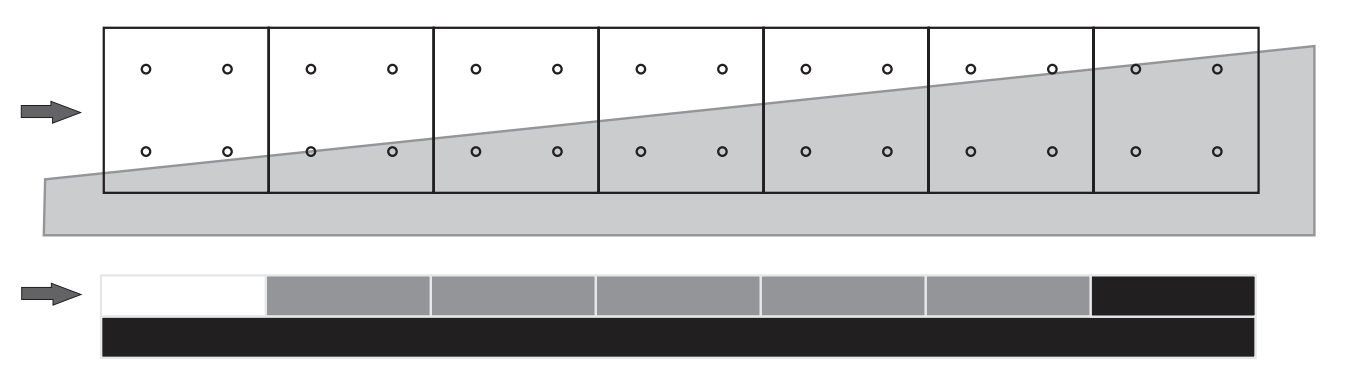
\includegraphics[width=\linewidth]{figures/ogss.png}
    \caption{Ordered Grid Super-Sampling\cite{Beets2000SupersamplingAA}}
    \label{fig:ogss}
\end{figure}

\section{Rotated Grid Supersampling}
\begin{figure}
    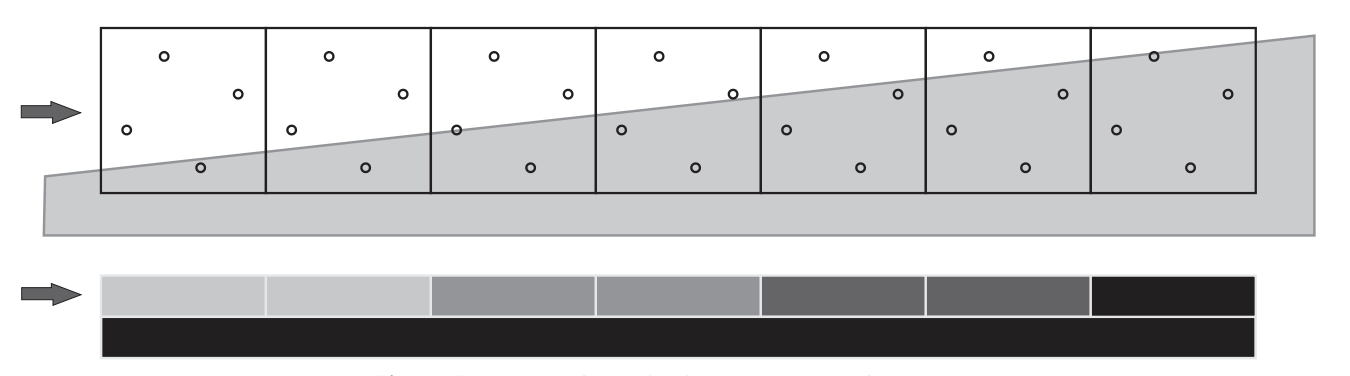
\includegraphics[width=\linewidth]{figures/rgss.png}
    \caption{Rotated Grid Super-Sampling\cite{Beets2000SupersamplingAA}}
    \label{fig:rgss}
\end{figure}

\section{Sparse Grid Supersampling}

\section{Multisampling}

\section{Post Processing Antialiasing}

Este tipo de antialiasing ha ganado popularidad durante los últimos años, debido en parte al uso del deferred shadin en los últimos motores gráficos. Este tipo de
fxaa detección de bordes
mlaa
smaa
%http://developer.download.nvidia.com/assets/gamedev/files/sdk/11/FXAA_WhitePaper.pdf
%https://software.intel.com/en-us/articles/morphological-antialiasing-mlaa-sample
%http://www.iryoku.com/smaa/
%http://www.iryoku.com/smaa/downloads/SMAA-Enhanced-Subpixel-Morphological-Antialiasing.pdf

\section{Temporal Antialiasing}

El temporal antialiasing es un tipo de antialiasing de post procesado, pero que amortiza el coste computacional usando multiples samples en multiples frames. Esto presenta unas complicaciones a la hora de escoger samples en frames anteriores en imagenes no setaticas.

\chapter{Temporal Antialiasing}

\chapter{Implementación de Temporal Antialiasing en Ugine}


% Bibliography:
\nocite{*}
\printbibliography{}

\listoffigures
\listoftables

% Index
\printthesisindex{}

\end{document}
